\section{Extensions}

\subsection{Memorizing Transformers}

\begin{frame}[c]{Memorizing Transformers}
    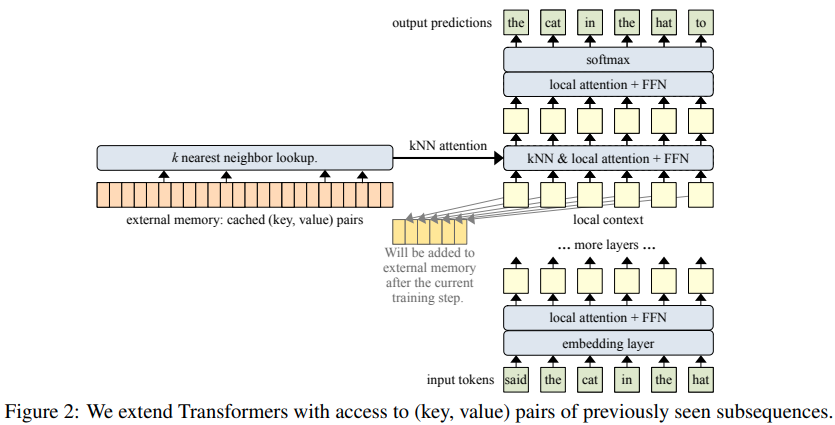
\includegraphics[width=\textwidth,trim=80 30 100 0,clip=true]{memorizing} \\
    \gray{Image Source: \cite{wu_memorizing_2022}}
\end{frame}


\begin{frame}[c]{Making a Model Memorize}
    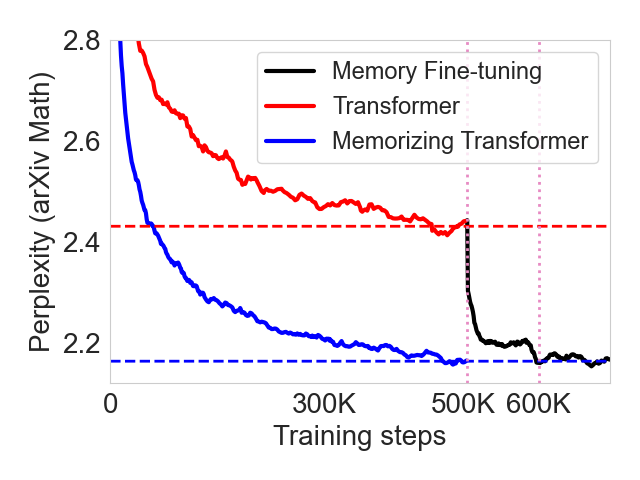
\includegraphics[height=0.8\textheight]{memorizing_bench} \\
    \gray{Image Source: \cite{wu_memorizing_2022}}
\end{frame}


\subsection{Vector Databases}

\begin{frame}[c]{Determining Nearest Neighbors in low dimensions}
    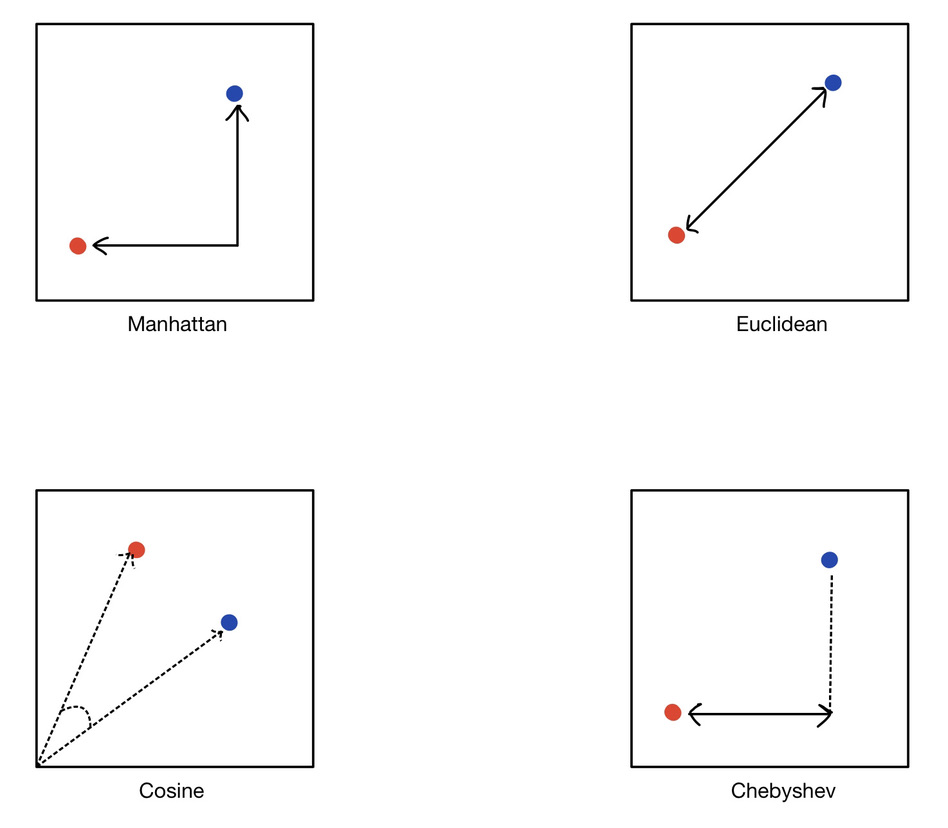
\includegraphics[height=0.8\textheight]{similarity-search-distance-metrics} \\
    \gray{Image Source: Public Domain}
    \pnote{
        No single metric is strictly better or worse \\
        But they are suited better or worse to certain tasks
    }
\end{frame}

\begin{frame}[c]{Vector Databases: Hierarchical Navigable Small World Graphs (HNSW)}
    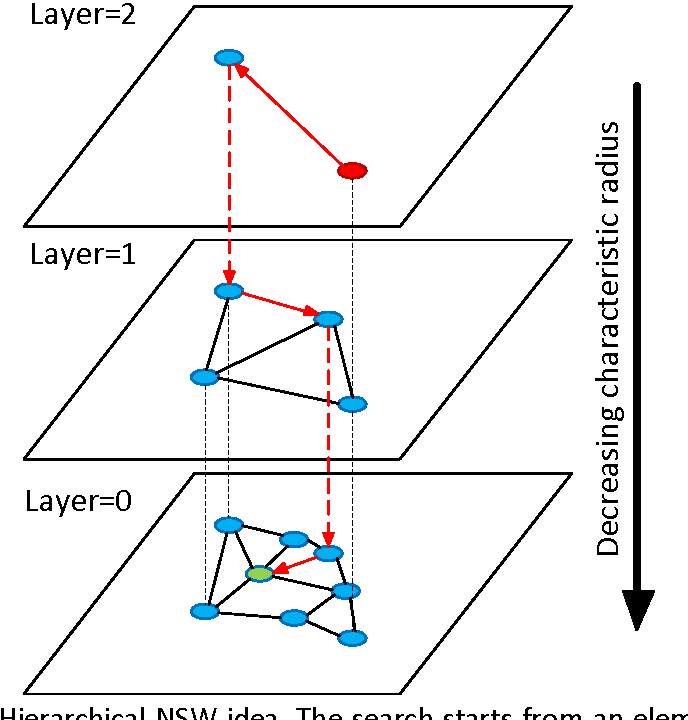
\includegraphics[height=0.7\textheight,clip=true,trim=0 15 0 0]{hnsw} \\
    \gray{Image Source: \cite{malkov_efficient_2020}}
    % (See e.g. \url{pinecone.io/learn/hnsw/} for more details)
    % Family of fast lookup vector index structures, optimized for such use cases

    % Hierarchical Navigable Small Worlds (HNSW)
\end{frame}


\begin{frame}[c]{HNSW SkipList Index Structures}
    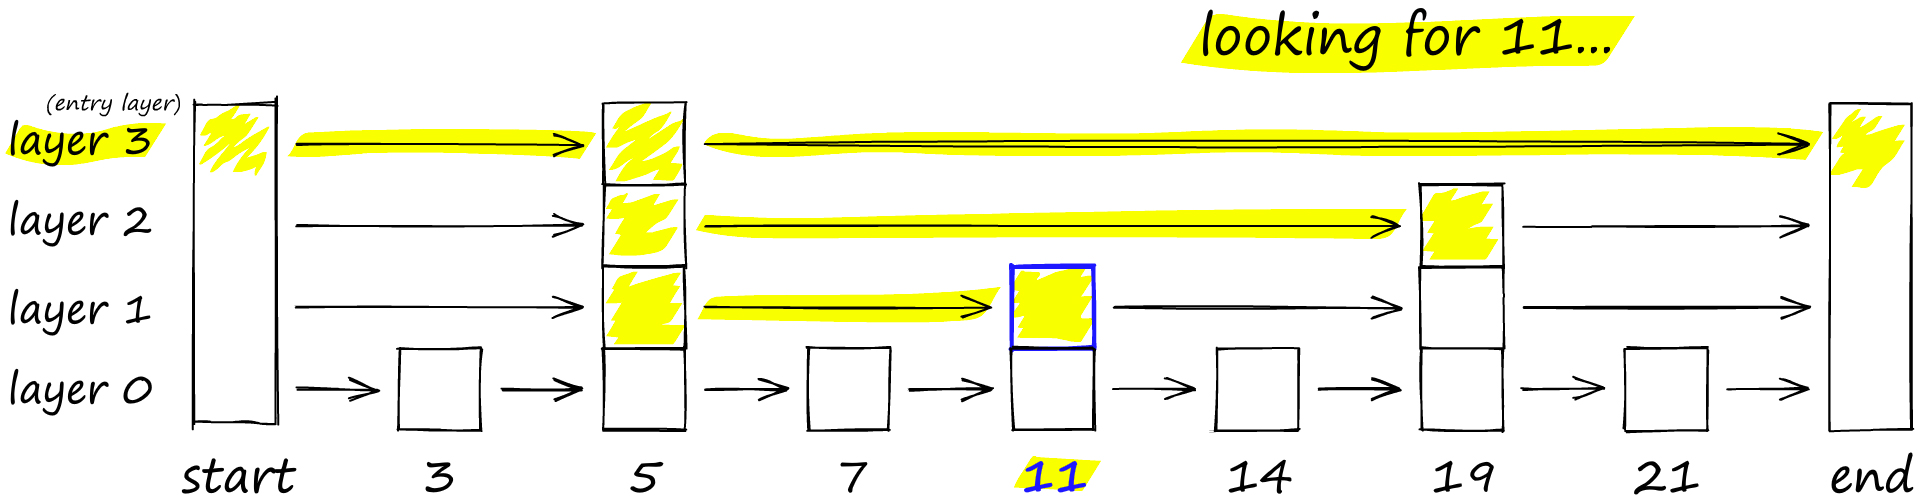
\includegraphics[width=\textwidth]{hnsw_skiplist} \\
    \gray{Image Source: \cite{pinecone_hierarchical}} 
\end{frame}

\subsection{Plugins}

\begin{frame}[c]{Plugins}
    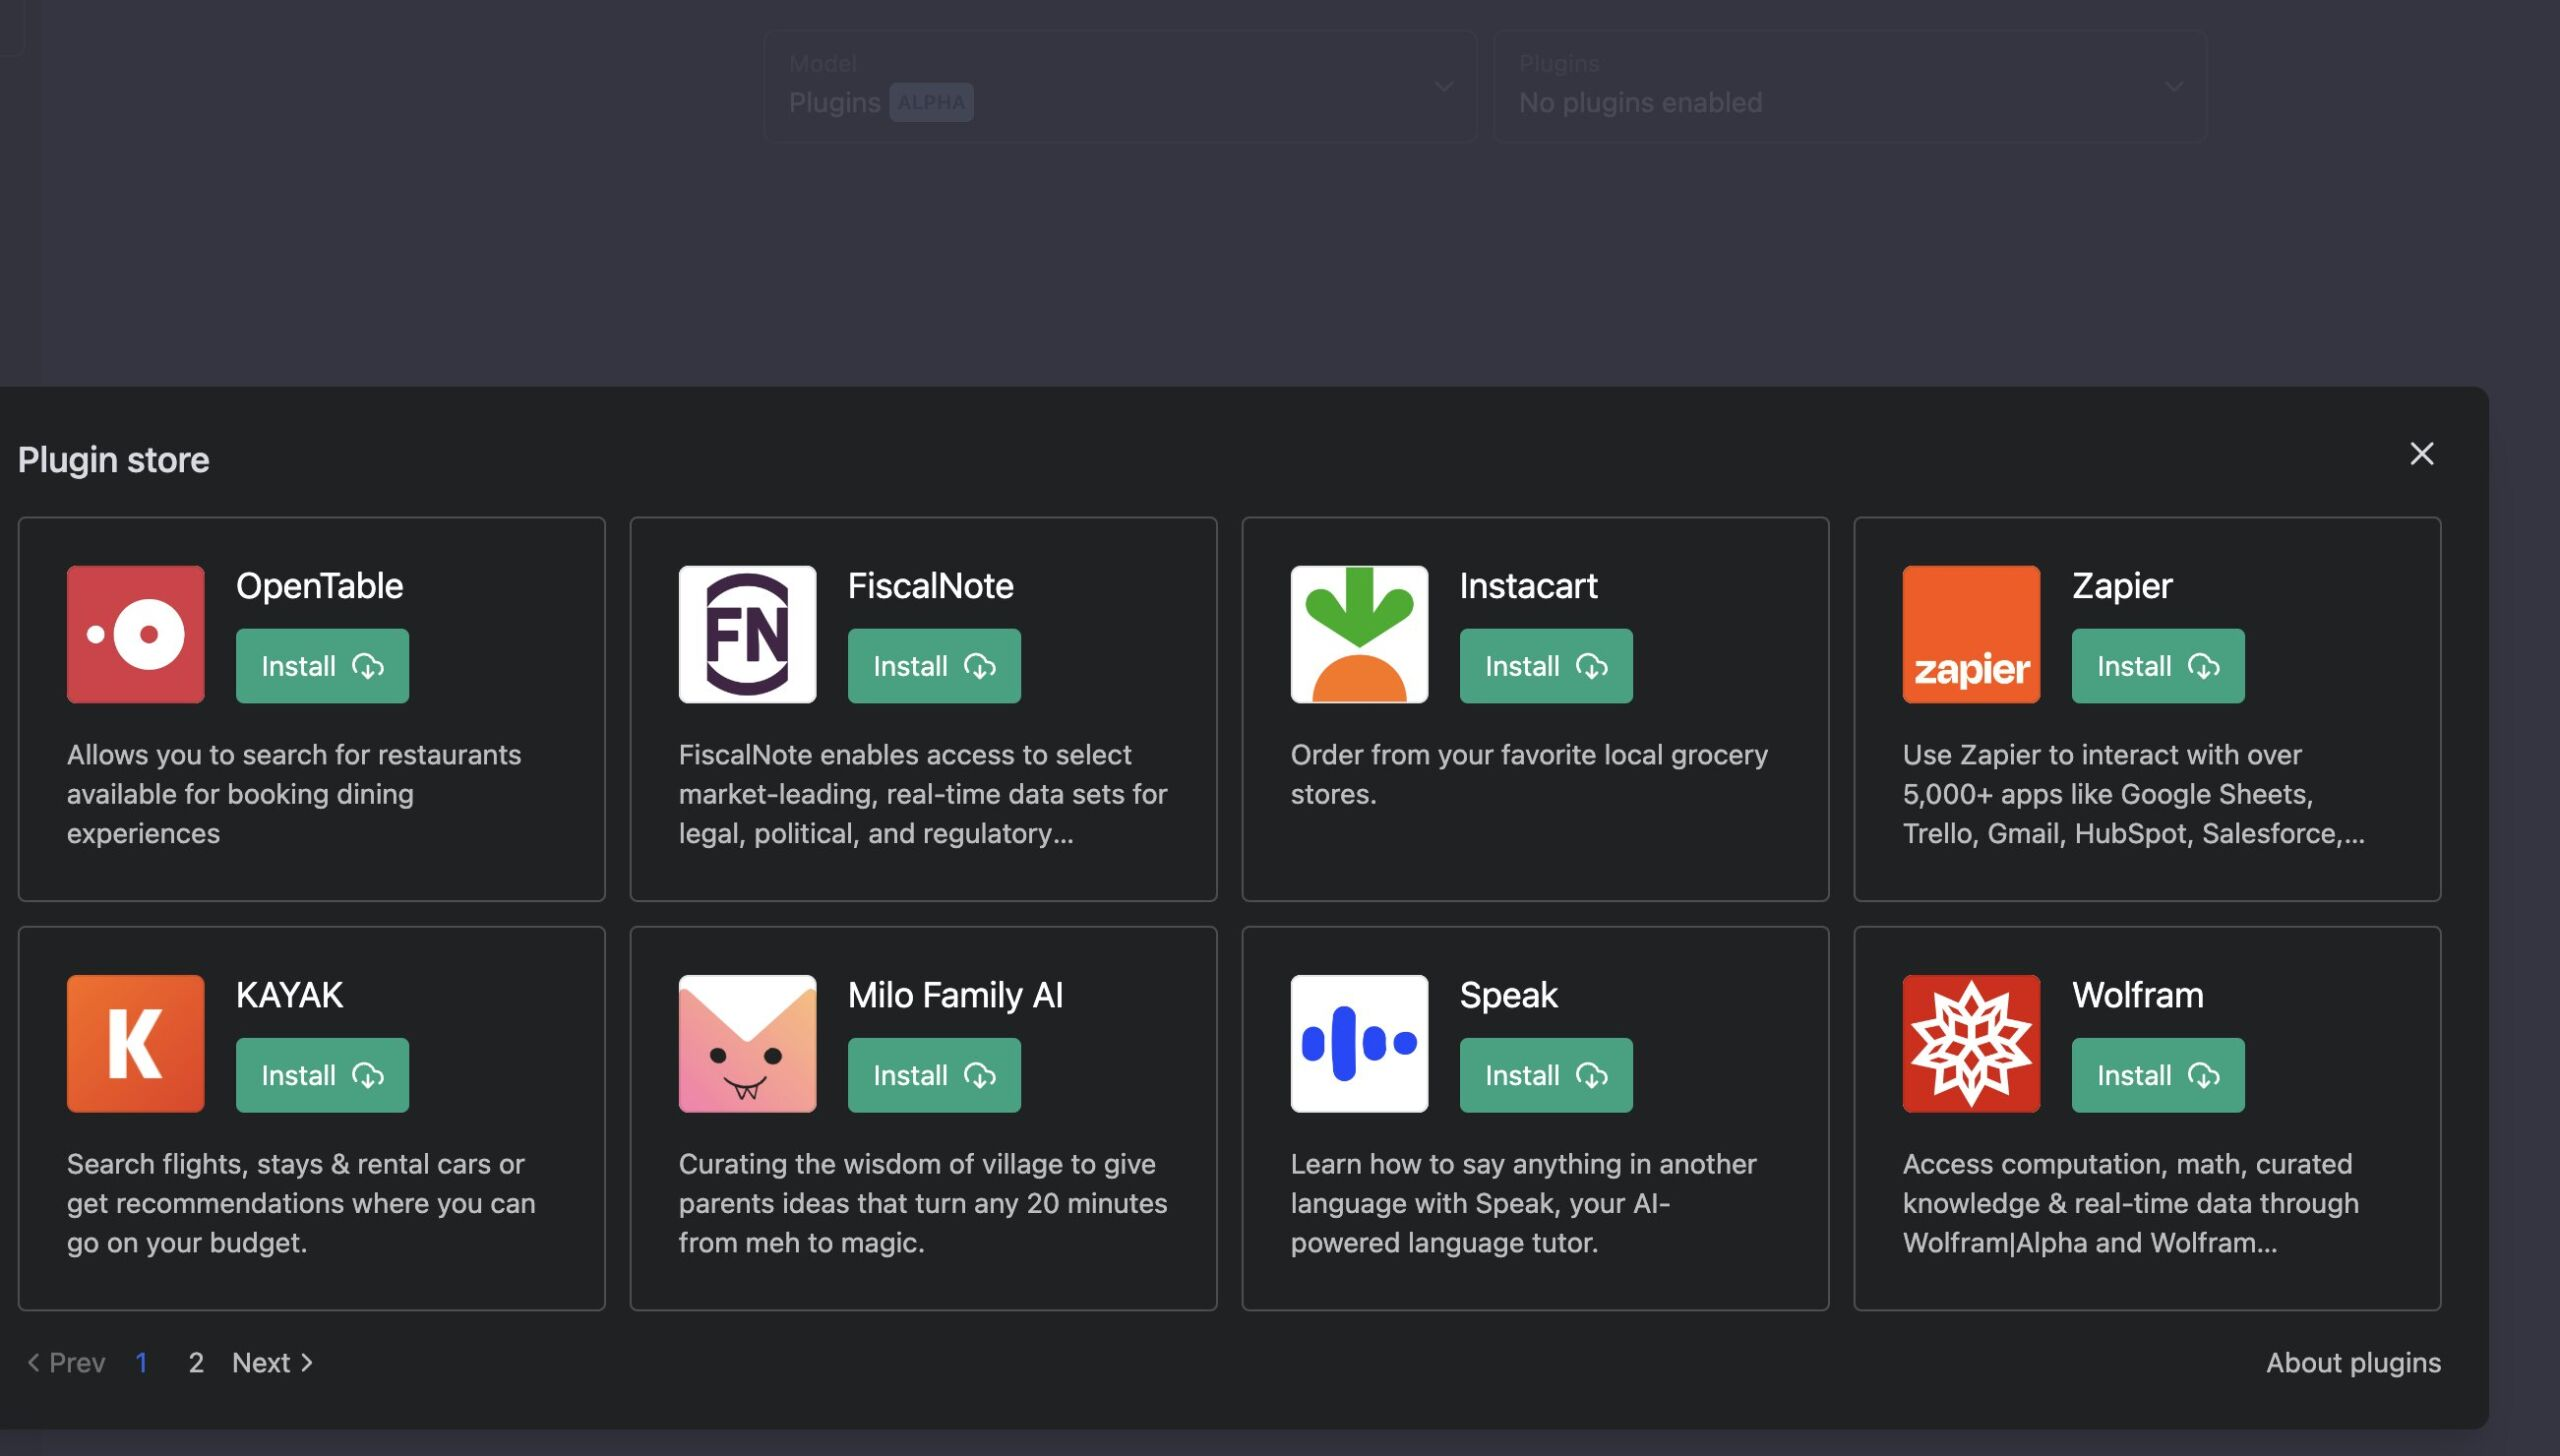
\includegraphics[width=\textwidth]{plugins}
\end{frame}


\begin{frame}[c]{Plugins II}
    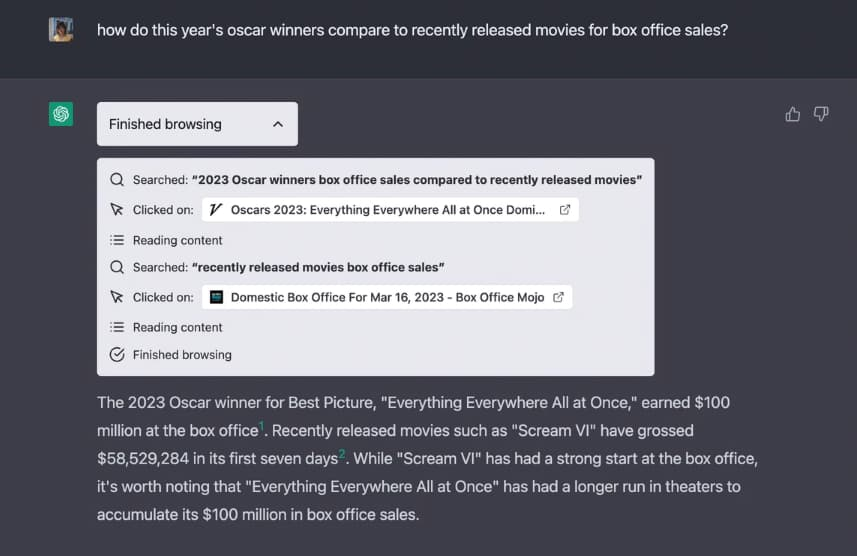
\includegraphics[width=\textwidth]{plugins-in-chatgpt}
\end{frame}


\subsection{Reflexion}

\begin{frame}[c]{Reflexion: Refining Answers with Self-Reflection}
    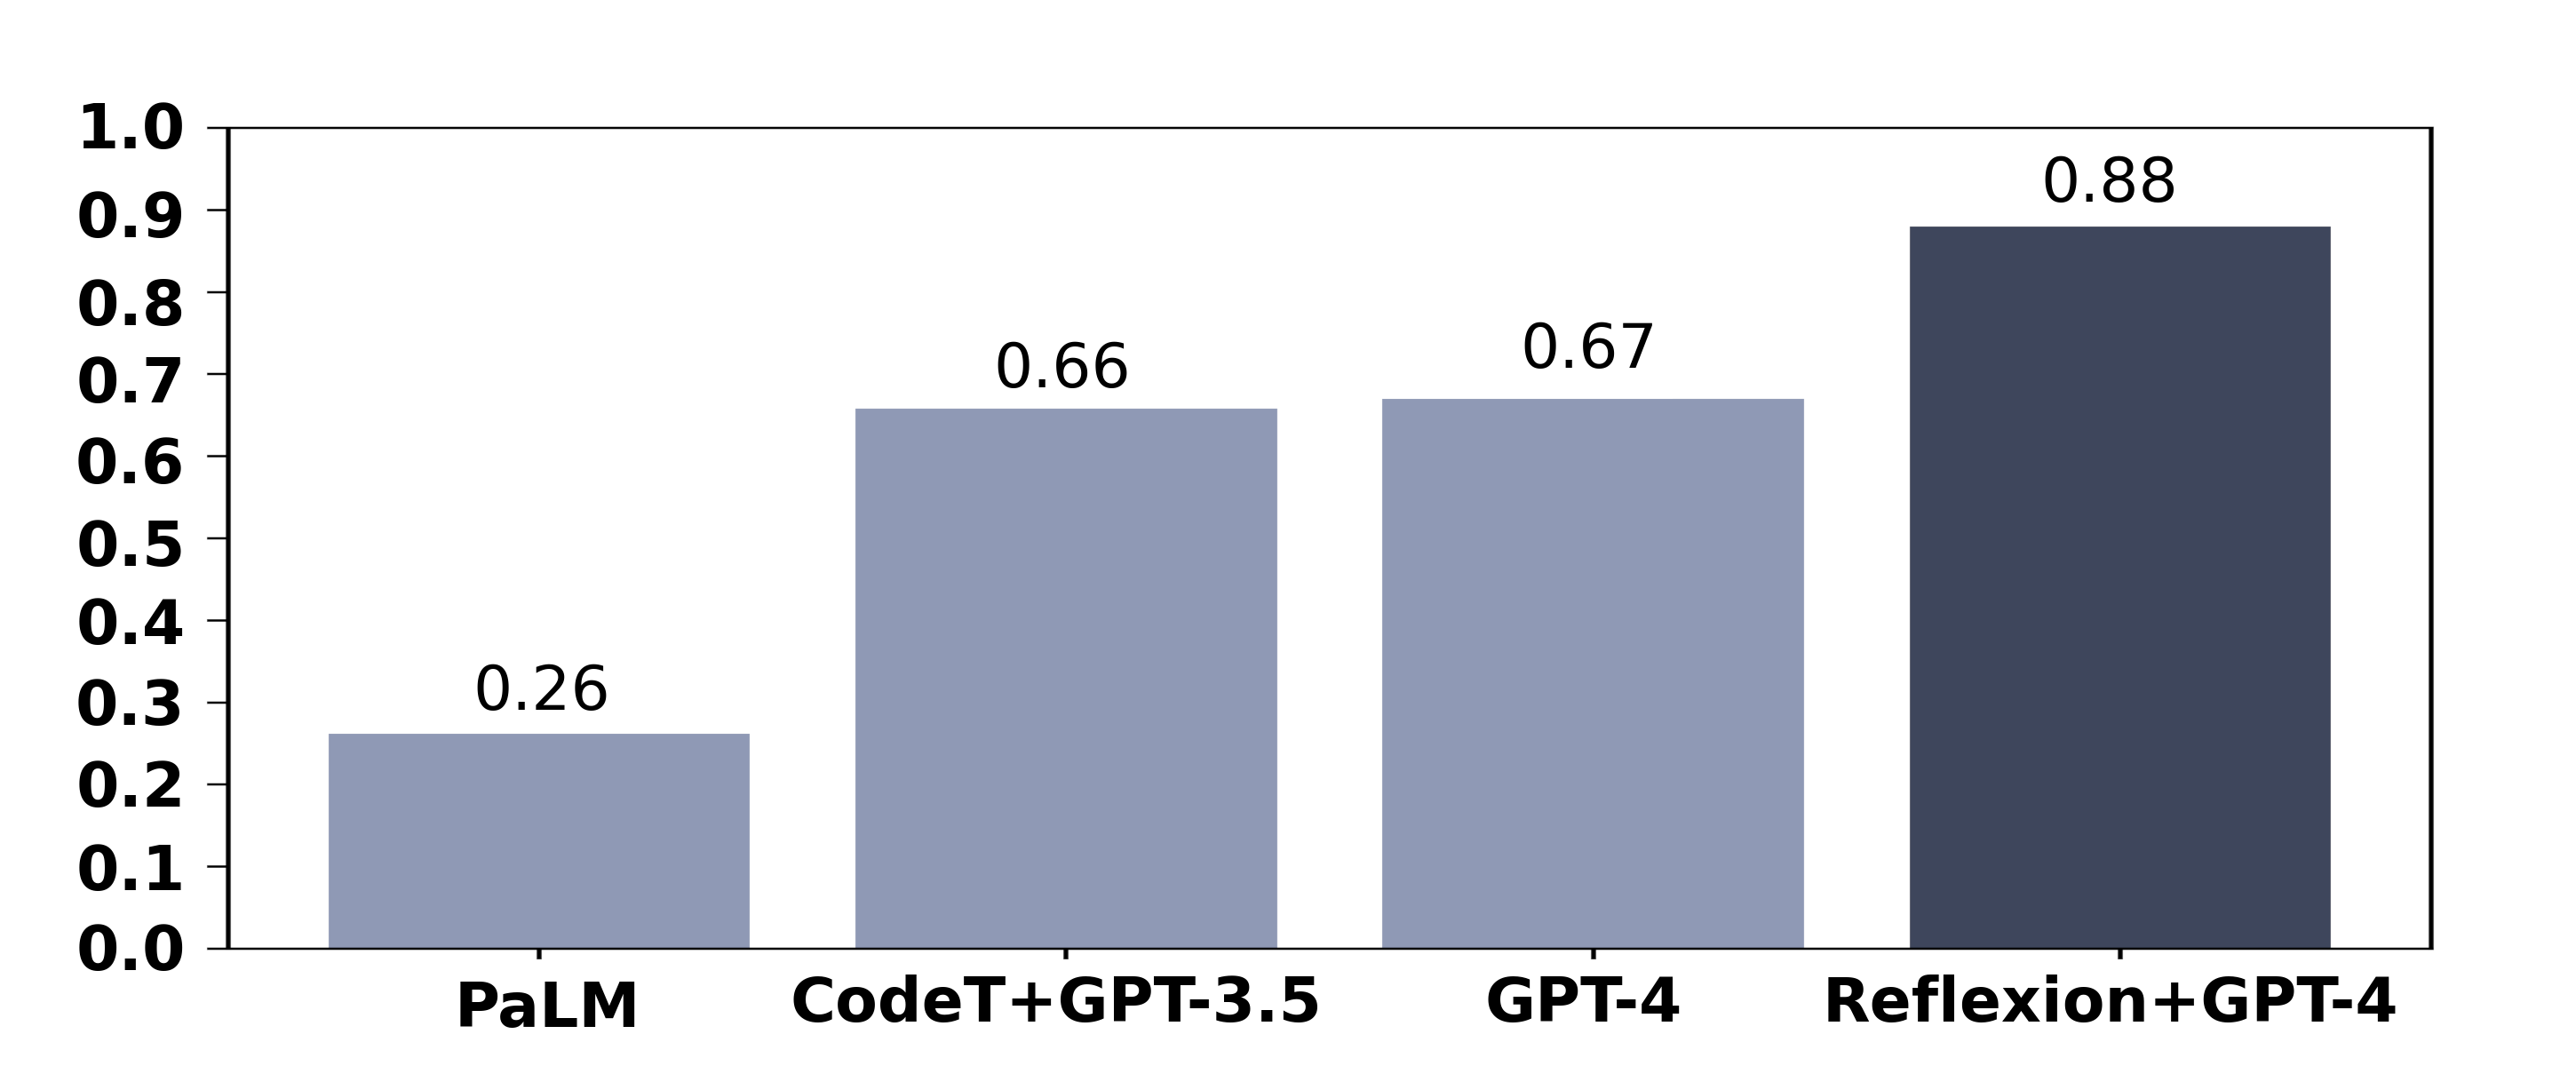
\includegraphics[width=\textwidth,height=0.43\textheight,trim=0 0 0 15,clip=true]{reflection_performance} \\
    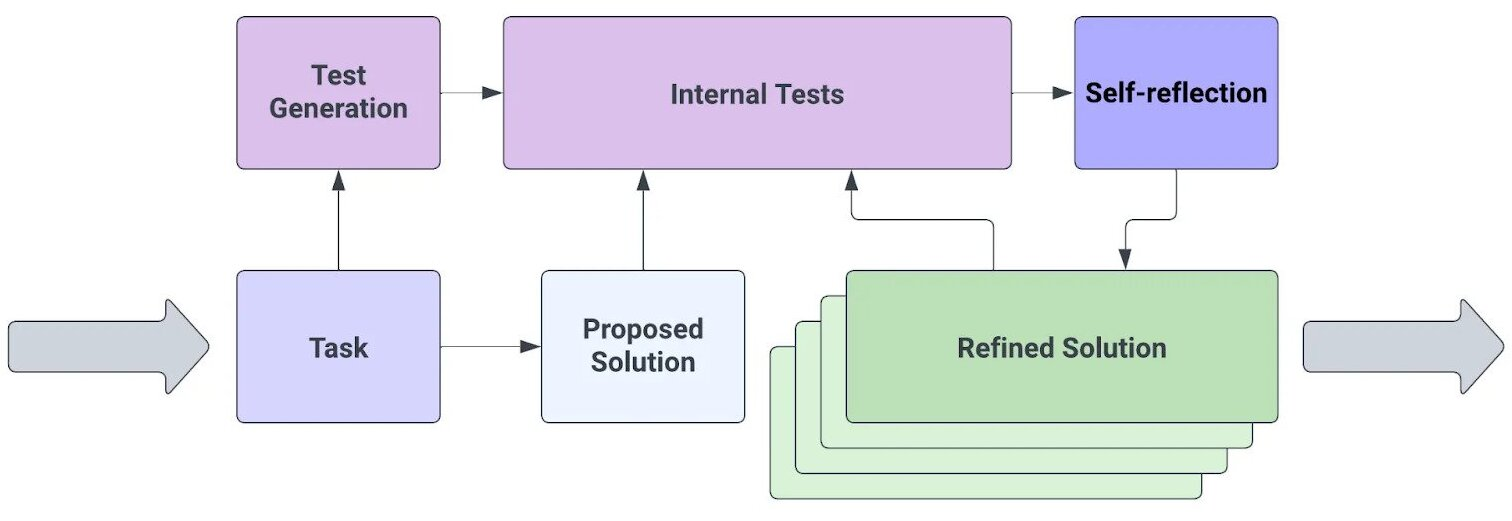
\includegraphics[width=\textwidth,height=0.38\textheight]{reflexion} \\
    \gray{Images Adapted from: \cite{shinn_reflexion_2023}} 
    \large
    ``is this correct actually?''
    \pnote{
        reflection improved performance on average
        from 67\% to 88\%, so by 200 basis points
    }
\end{frame}

\subsection{AutoGPT}
\begin{frame}[c]{AutoGPT: Multi-Shot Reflection on Steroids}
    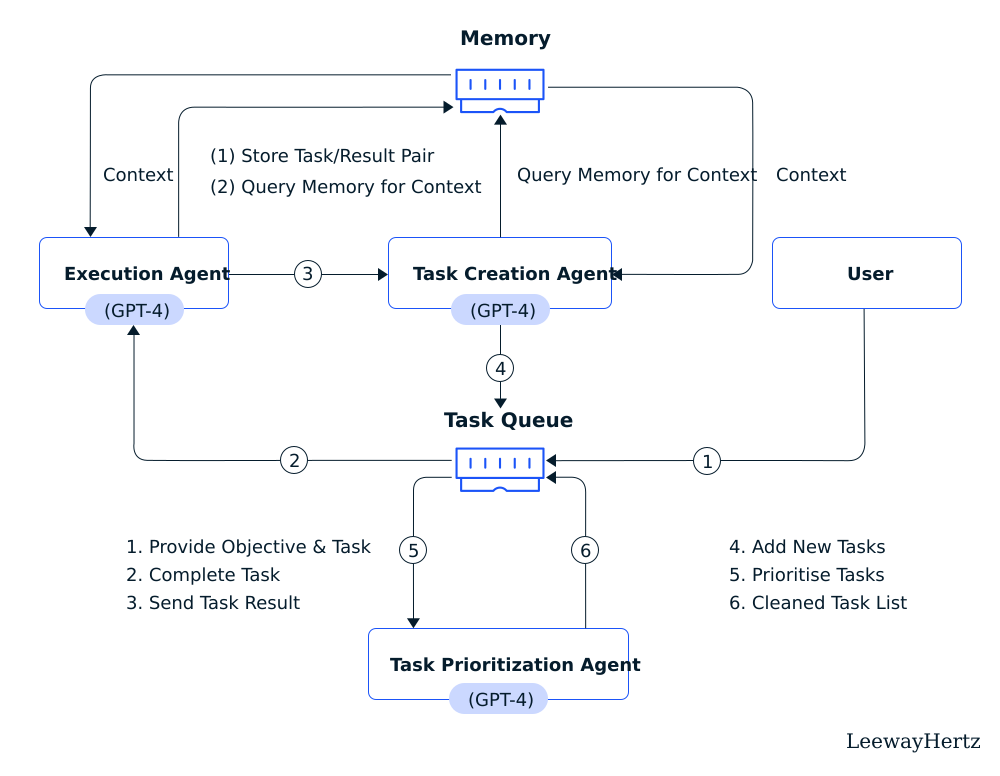
\includegraphics[height=0.8\textheight]{autogpt} \\
    \gray{Project Source: \cite{significantgravitas_2023}}
    \pnote{
        iteratively using goal-directed reflection \\
        and all plugins available to split and solve \\
        more complicated tasks.
    }
\end{frame}

\subsection{Interactive Simulacra}
\begin{frame}[c]{Interactive Simulacra of Human Behavior}
    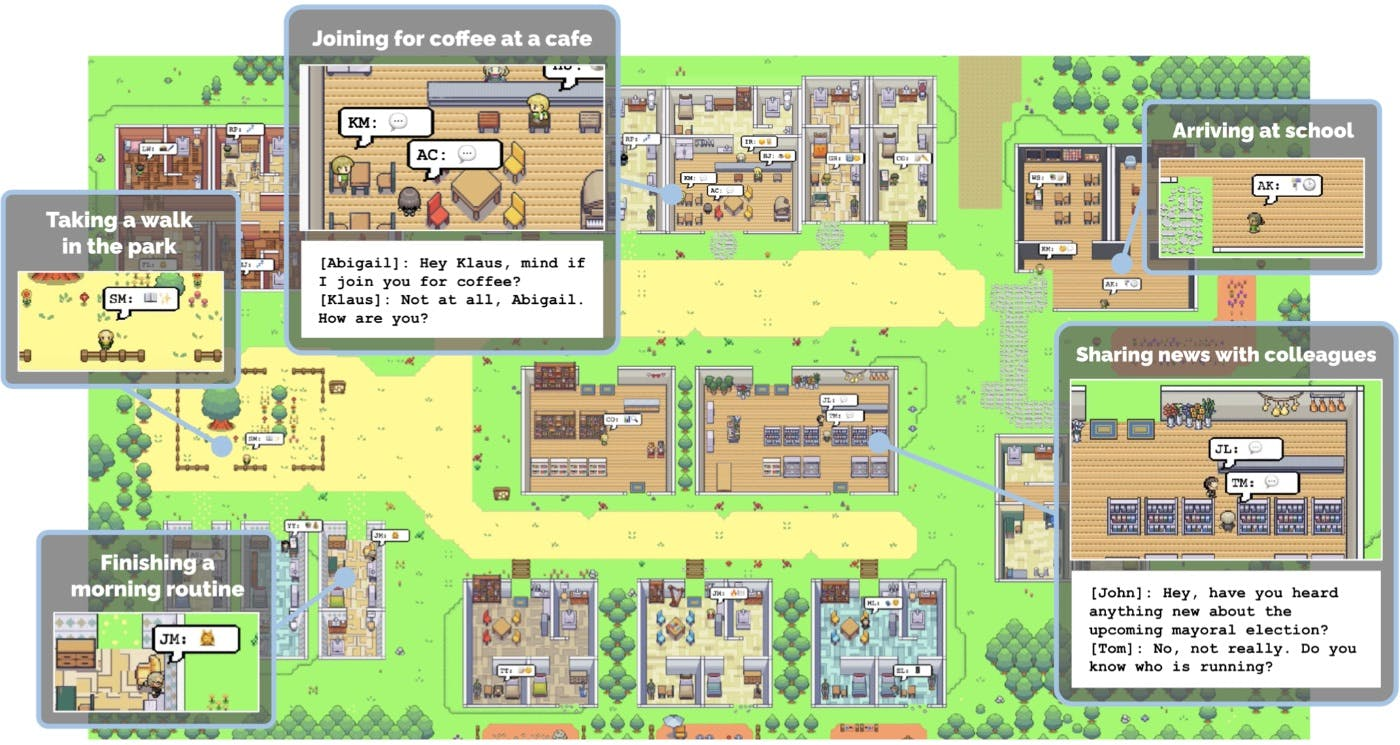
\includegraphics[width=\textwidth]{simulacra} \\
    \gray{Image Source: \cite{park_generative_2023}}
    \pnote{
        Simulated agents managed to coordinate \\
        going to a party and build relationsships.
        \\
        They also had a follow-up paper, \\
        though I haven't read it in detail
    }
\end{frame}


\begin{frame}[c]{Simulacra Architecture}
    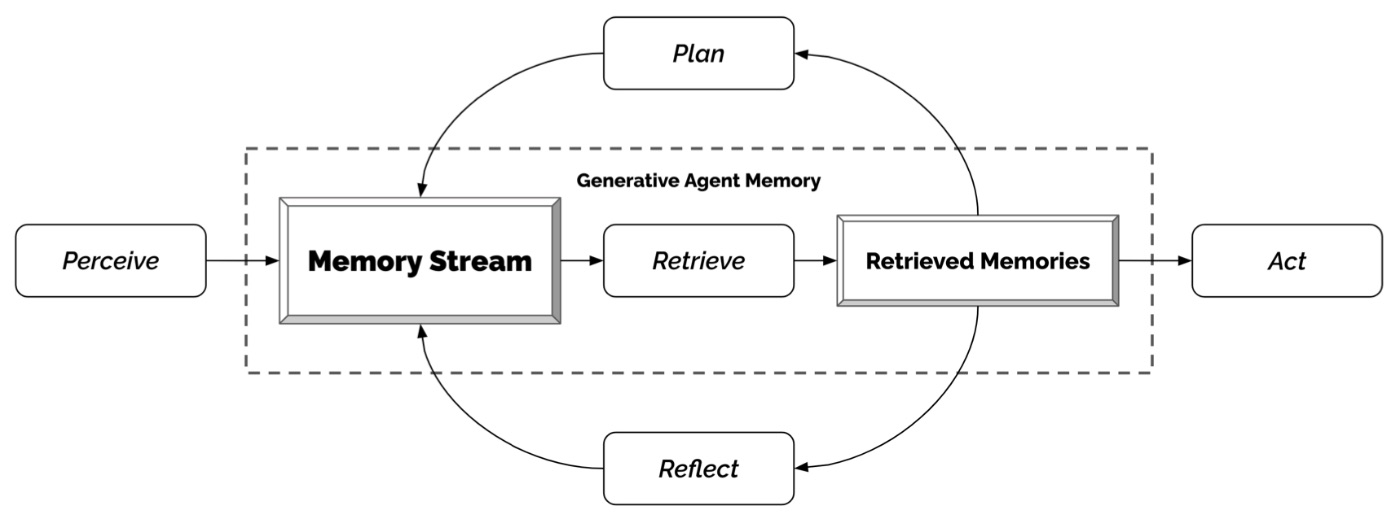
\includegraphics[width=\textwidth]{simulacra_arch} \\
    \gray{Image Source: \cite{park_generative_2023}}
\end{frame}

\subsection{Fine-Tuning}
\begin{frame}[c]{InstructGPT: Following Instructions}
    \begin{aquote}{Ouyang et. al. 2022 \cite{ouyang_training_2022}}
        In human evaluations on our prompt distribution, outputs from the 1.3B
        parameter InstructGPT model are preferred to outputs from the 175B
        GPT-3, despite having 100x fewer parameters. Moreover, InstructGPT
        models show improvements in truthfulness and reductions in toxic output
        generation while having minimal performance regressions on public NLP
        datasets.
    \end{aquote}
    \pnote{
        You had to write 'a good list of .... would be:' before that
    }
\end{frame}

\begin{frame}[c]{Reinforcement Learning from Human Feedback}
    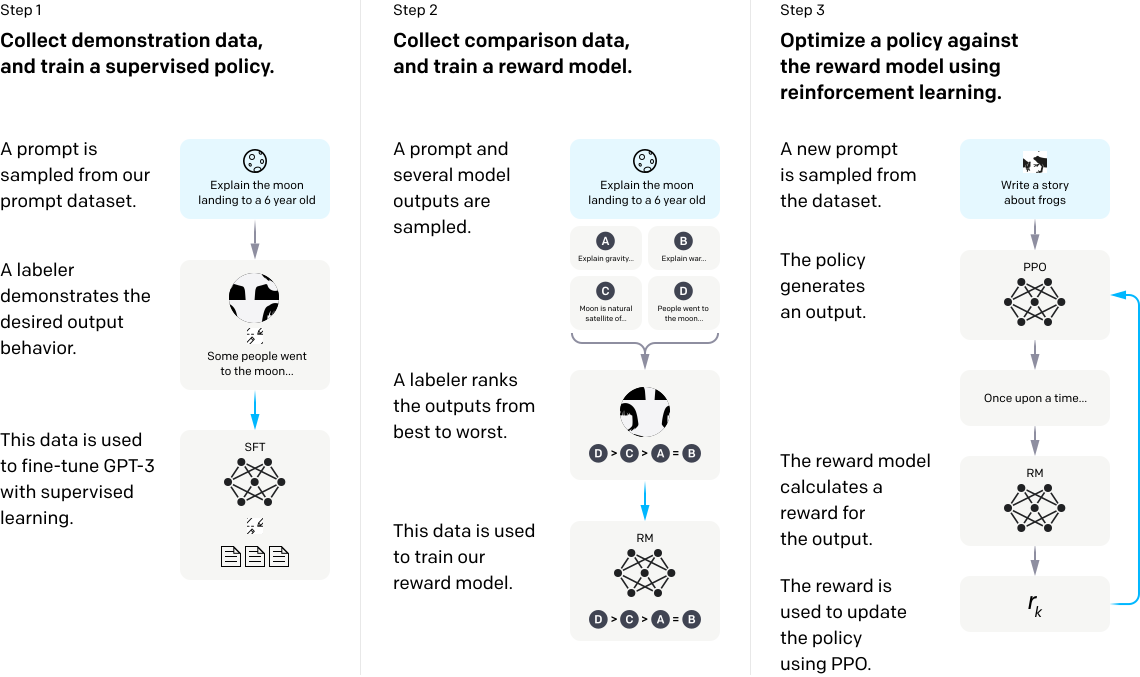
\includegraphics[height=0.8\textheight]{instruct}\\
    \gray{Image Source: \cite{ouyang_training_2022}} \large \hspace{2em} RLHF originated from \cite{christiano_deep_2017}
\end{frame}

\begin{frame}[c]{ChatGPT}
    
\includegraphics[height=0.8\textheight]{chatgpt} \\
    \gray{Image Source: \cite{chatgpt_2023}}
\end{frame}

\begin{frame}[c]{ChatGPT Training Steps}
    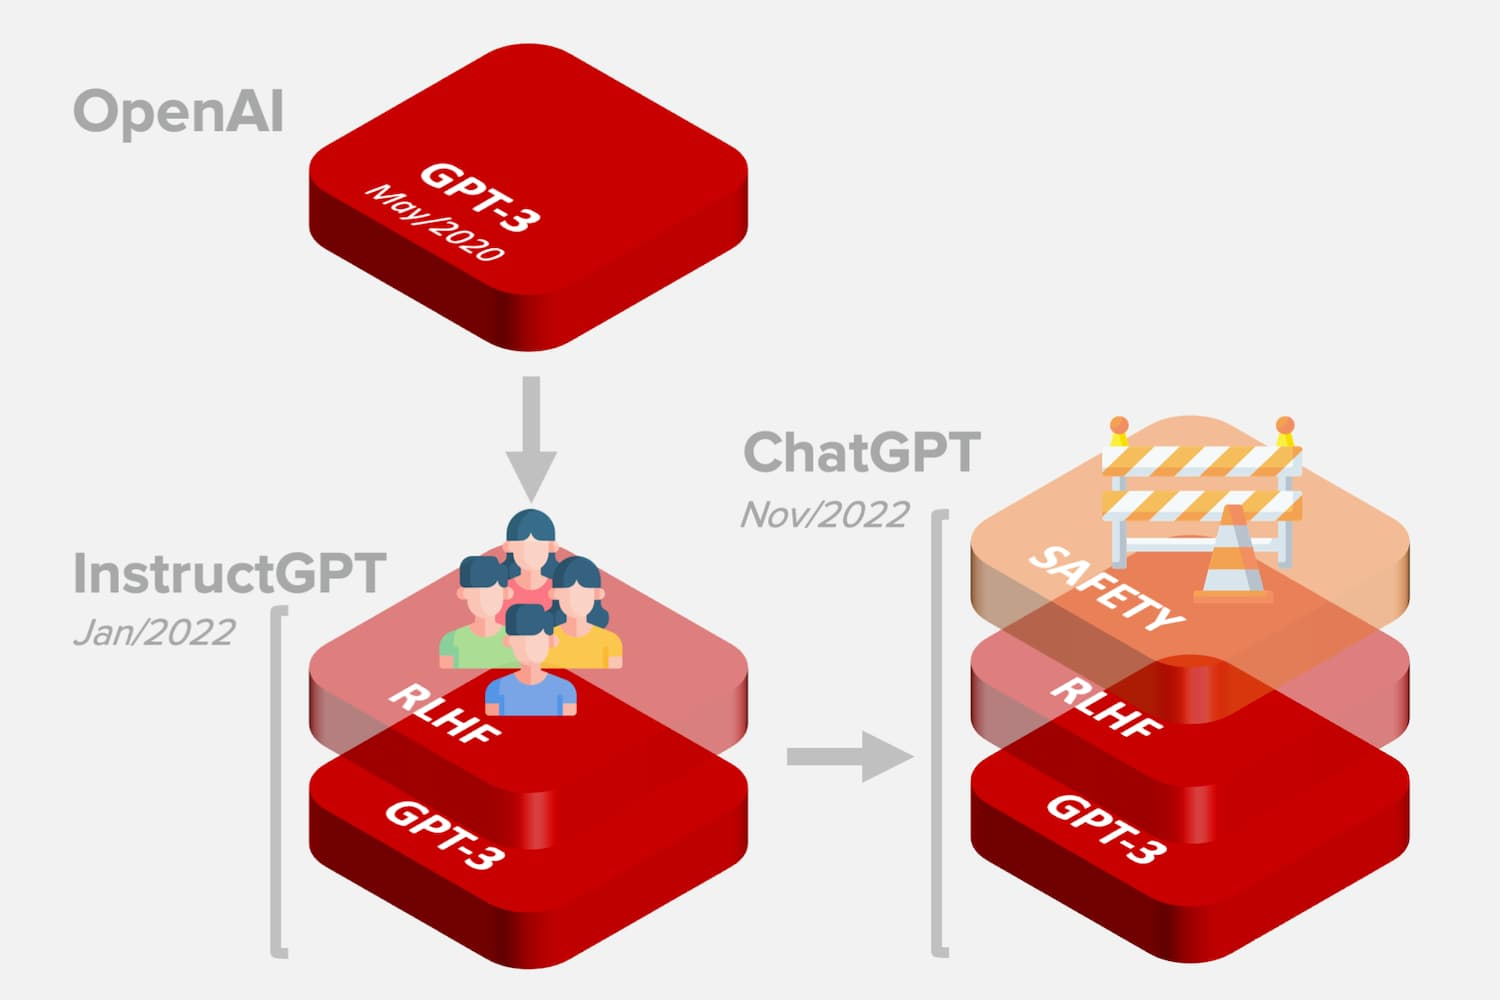
\includegraphics[height=0.8\textheight]{chat_instruct} \\
    \gray{Image Source: \cite{what_2023}}
    \pnote{
        Technically speaking often Instruct=RLHF but eh\\
        \\
        ChatGPT is thus a 'lobotomized', \\
        less useful version when compared to the original InstructGPT
    }
\end{frame}


% \begin{frame}[c]{Constitutional AI} 
%     \begin{enumerate}[<+(1)->]
%         \item The AI answers many questions, some of which are potentially harmful, and generates first draft answers.
%         \item The system shows the AI its first draft answer, along with a prompt saying “rewrite this to be more ethical”.
%         \item The AI rewrites it to be more ethical.
%         \item The system repeats this process until it collects a large dataset of first draft answers, and rewritten more-ethical second-draft answers.
%         \item The system trains the AI to write answers that are less like the first drafts, and more like the second drafts.
%     \end{enumerate}
% \end{frame}

\begin{frame}[c]{Constitutional AI}
    \large
    \begin{enumerate}[<+(1)->]
        \item Prompt LLM with questions illiciting ethically questionable responses
        \item Ask it to "rewrite this to be more ethical"
        \item Fine-Tune to prefer rewritten response
        \item Repeat a few times
    \end{enumerate}
\end{frame}

\begin{frame}[c]{Constitutional Results}
    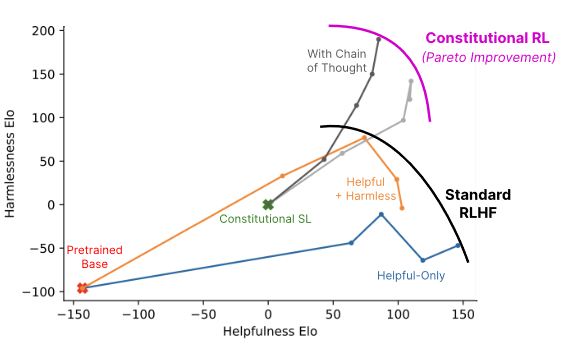
\includegraphics[height=0.8\textheight]{constitutional_benchmark} \\
    \gray{Image Source: \cite{bai_constitutional_2022}}
    \pnote{
        The model uses the ethics it learned implicitly. \\
        Not sure if this creates additional problems
    }
\end{frame}

